\documentclass{standalone}
\usepackage{tikz}
\usepackage{ctex,siunitx}
\setCJKmainfont{Noto Serif CJK SC}
\usepackage{tkz-euclide}
\usepackage{amsmath}
\usetikzlibrary{patterns, calc,3d}
\usetikzlibrary {decorations.pathmorphing,decorations.pathreplacing,decorations.shapes}
\begin{document}
\small
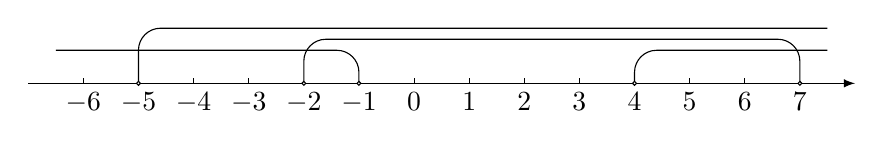
\begin{tikzpicture}[>=latex,scale=0.7]
  \draw[->](-7,0)--(8,0);
  \draw(-2,0)--(-2,0.4)arc(180:90:0.4)--(6.6,0.8)arc(90:0:0.4)--(7,0);
  \draw(-1,0)--(-1,0.2)arc(0:90:0.4)--(-6.5,0.6);
  \draw(4,0)--(4,0.2)arc(180:90:0.4)--(7.5,0.6);
  \draw(-5,0)--(-5,0.6)arc(180:90:0.4)--(7.5,1.0);
  \foreach \x in {-5,-2,-1,4,7}
    {\draw[fill=white](\x,0)node[below]{$\x$}circle(1pt); }
  \foreach \x in {-6,-4,-3,0,1,2,3,5,6}
    {\draw[very thin](\x,0)node[below]{$\x$}--(\x,0.1);}
\end{tikzpicture}
\end{document}